\chapter{Architecture}
\label{cha:architecture}

\dots

\section{Solution design}
\label{sec:design}
This section describes the specifications of the functionalities of the system. Each functionality is a logical group of actions whose purpose is to carry out a section of the job required to go from row data - a user identifier - to a piece of information - the answer to the question "Has this person lived a life event?". The steps are the following:
\begin{enumerate}
\item Collect activities from social networks.
\item Extract semantic entities from social network contents.
\item classify each content.
\item Decide whether the user has lived the life event relying on his/her contents.
\end{enumerate}
In the following subsections the logic of the proposed methodology will be illustrated.

\begin{figure}
\centering
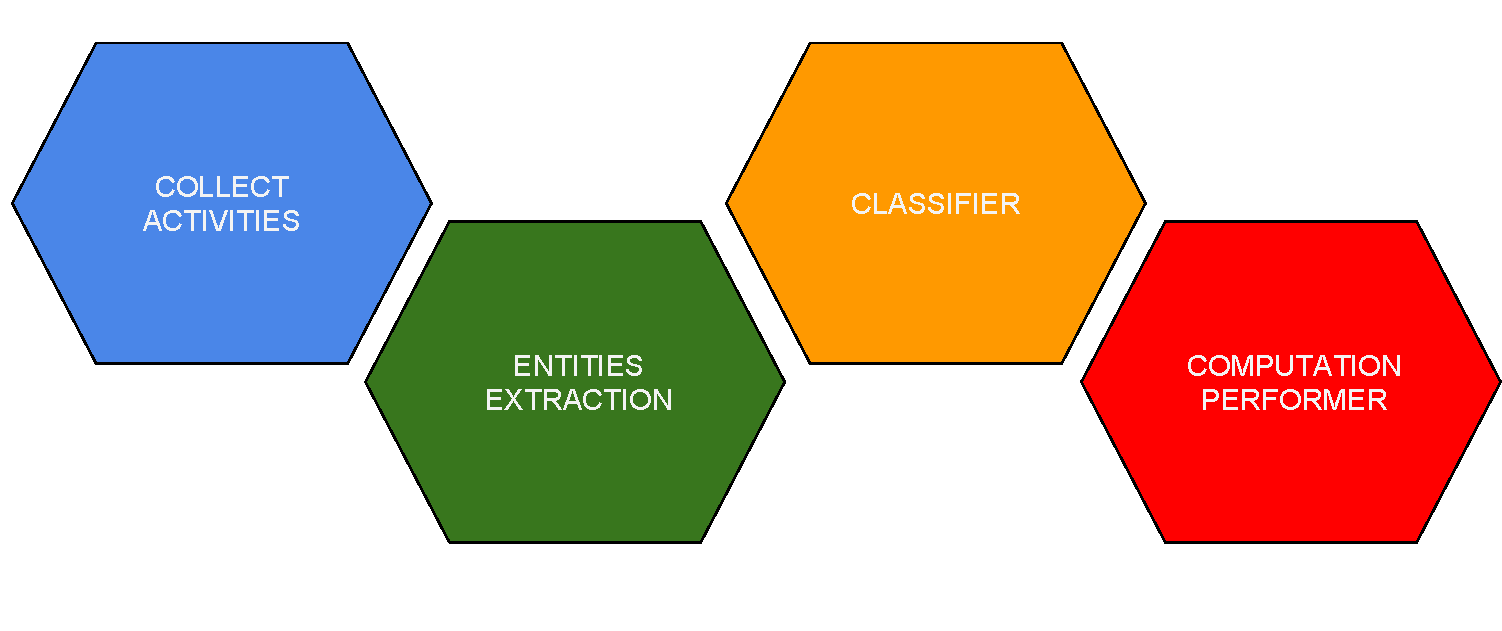
\includegraphics[width=%
0.8\textwidth]{img/Solutiondesign_nutshell}
\caption{The solution design in a nutshell.}
\label{fig:nutshell}
\end{figure}

\subsection{Collect activities}
This part has the goal to fetch user's contents on social networks, using the services for developers offered by the official APIs of each social network. The data of interest are some pieces of user's information, such as name, birthday, number of friends/followers, subscription date, his/her location and language, and of course all his/her contents: all the posts he/she wrote, with attachments, external links and the publication date, with also some other useful metadata, such us the number of likes, replies and shares.

As input this functionality needs a series of IDs that identify the user among all the social networks he/she uses, and for each social platform is necessary to know at which point the data of a given user has been downloaded. In fact, due to the huge amount of data, social network services return a small quantity of data for each request, therefore, after the first one request, the point from which start to download data must be specified.

As output, a list with \textit{new} user's post is expected. In case it's the first time that the data of a user is downloaded, a list of user's information is expected too, otherwise $ n $ new posts are enough. The term \textit{new} means that all the fetched post were not previously downloaded by the system, turning out to be new for it, even if they can be dated far in the past. In other words, a new post for our system may not be new for the social network, but is simply a post that were not included in any of the previous download for that given user. Last but not least, the point the data has been fetched for the user must be updated.

The number $ n $ of post to download could be given as parameter. It would be better if the number is \textit{small}, not to overload the system. For example, Twitter allows to fetch up to $ 200 $ tweets a request. The default parameters should be setted equal to the maximum limit imposed by the API.

\subsection{Entities extraction}
This part has the task to add semantic information to the data that was previously downloaded from social networks. What is obtained from the previous part are only raw texts and images, the goal is now to understand what the user has talked about into his/her posts. To do that, some external semantic analyzer will be used: this kind of service extracts entities, topics and sentiment starting from a text or a image.
An \textit{entity} is a person, an object or a concept that has an article on Wikipedia; a \textit{topic} is a Wikipedia category to which an entity belongs to. For example, the phrase "I'm studying computer science at the university" has two entities - \texttt{Computer science} and \texttt{University} - and the following list of topics: \texttt{Electrical engineering, Electronic engineering, Computer engineering, Computer science, Educational stages, Higher education, Types of university or college, Universities and colleges, Youth}. These new metadata added to the information obtained previously will be useful in further steps to understand whether a post is about a life event or not. This functionality has also the delicate task to deal with the request rate limits of the external analyzers: in fact many of these API have strict limitations for free plans, allowing only a small amount of requests in a certain time window. In case the limit runs out, this part of the system has to suspend himself waiting for another time window to send new requests, keeping in memory all the computation requested in the meantime.

A post, composed by text, images or external links is expected as input. Furthermore, a list of posts could be accepted as input, but in this case the number of remaining requests must be handled carefully.

As output, a list of entities, topics and sentiment scores is returned for each post analyzed. The sentiment score is made by a floating point number, that ranges from a minimum value - such as $ -1.0 $ - to a maximum value - like $ 1.0 $. Instead, entities and topics can be represented by a string or an \texttt{URI}, for example a \texttt{Wikipedia URI}.

By default, everything that is returned by the external analyzer could be given as output, together with a confidence for each entity found inside texts or photos. In addition, this part of the system should provide the possibility to consider only the \textit{top entities} (e.g. the most meaningful, or those with the highest confidence), and also the possibility to set a minimum value of confidence under which the entity is discarded.

\subsection{Classifier}
This part has the fundamental purpose to decide whether a post is about or not to a certain life event. Its task is to extract some features from the posts previously downloaded, and apply some machine learning algorithm to take this decision.

At this point the current situation is, for each user taken into analysis, a list of posts - made by texts, attachments and images - enriched with semantic entities, topics and sentiment score. The input will be a tuple made by a post, composed as just described, and a life event of interest, for which we want to predict if the post is about it. A life event could be represented by an unique string, e.g. "\texttt{GETTING\char`_MARRIED}" for a wedding, or alternatively by an integer ID.

As output, a label indicating "Y" or "N" is expected (of course "Y" in case the post is about the life event, otherwise "N"). In addition, an estimation of the reliability of the result could be returned.

The feature extraction method can be decided a priori, or it can be setted as parameter: using only \textit{text features} - the words that compose the text of each post - or use only \textit{entity features} - the semantic entities for reasoning on the meaning of the post, or use them both together. This choice should be made paying attention to the available datasets to train the classifier: in fact, if \textit{text features} are chosen, at least a different dataset for each language supported has to be provided.

\subsection{Computation performer}
This last function has the goal to analyze the user's timeline to discover a life event in it. Since a life event is something important and rare into a user's life, the assumption is that also in his/her social life his/her behaviour is different when the event is approaching or is in progress. For this reason some unusual patterns, related to the life event itself or to the average success of the posts, are searched for. The idea is that a user does not publishes contents about, for examples, a new baby, very usually, but only when something important is about to happen. In addition to that, a post about a new baby announcement gets probably more feedbacks compared to a normal post, such as congratulation messages. The detection of a life event is based on these routine changes, which can be various: a slow but constant increase of interest before the event, or a sudden peak when the event is happening. In general, the relative frequency of activities related to the life event itself is monitored.
At this point, a timeline is composed by a list of Y/N label, each one with a timestamp attached. For each day $d$ the user has been active on social media (those days in which the user published something), the frequency $f$ is computed as follows:
\[
f(d) = \frac{r(d)}{all(d)}
\]
where $r(d)$ is the number of posts related to the life event written the day $d$, and $all(d)$ is the count of all posts published the day $d$. Of course, the timeline is already targeted with the life event taken into consideration. In other words, the life event to monitor is chosen in the previous steps: at this point the timeline is labelled only for a single life event. Once the frequency has been computed for every day, it can be plotted over time, and at the moment $f$ passes a given threshold $\alpha$, the life event is begun. When a minimum number of days $\beta$ in which $f(t) > \alpha$ are found, the life event can be considered as detected. By the time in $\gamma$ days there are no \textit{active days}, the life event can be seen as over.

As input is expected a list of boolean label with a timestamp, that represents the user's timeline in function to a life event.

As output, a boolean answer is expected, together with a time range in which the life event has been detected (this range can be composed by the date of the first and the last post related to the life event). Of course, the user may have not lived the life event, so in this case the list will be empty. Also, a person can live a life event more than once, so the output can be a list of labels.

There are several parameter for this phase: 
\begin{itemize}
\item the threshold $\alpha$ for the frequency $f$ over which the life event is considered as started.
\item $\beta$, the minimum number of \textit{active days} to consider a life event detected. This parameter serves to correct any errors in post classification. In fact, is possible that a text or an image is misclassified: using this parameter is possible to avoid single and isolated errors.
\item $\gamma$, the maximum time between two \textit{active days} to consider them as related to the same life event. This parameter has the role to put an end to a detection, and consequently to split two consecutive life events.
\end{itemize}

\section{Exposed APIs}

TBD properly.

In linea di massima: 1) esiste l'utente X? 2) Aggiungi l'utente X 3) Scarica l'ultimo mese/settimana dell'utente X 4) L'utente X ha vissuto il life event Y (con i dati presenti)?

\section{Global view}
